
\documentclass{beamer}
\usepackage{tikz}
\usetikzlibrary{positioning,calc,arrows.meta}

\begin{document}

	\begin{frame}{GPIO Read Subroutine Execution}
		\centering

		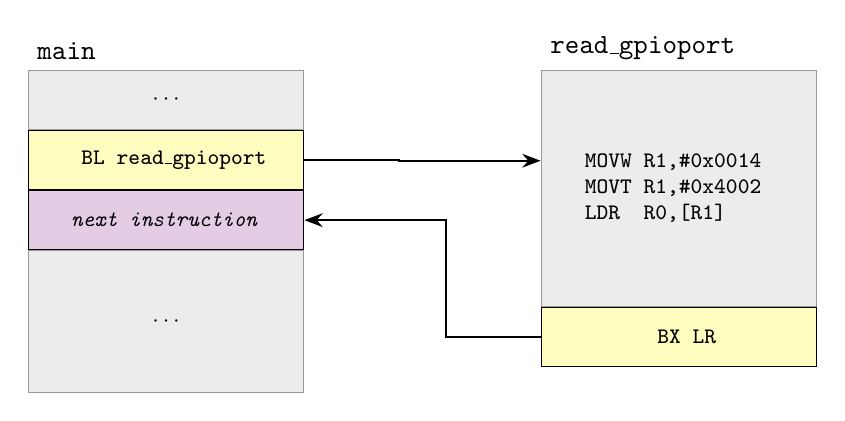
\begin{tikzpicture}[
			>=Stealth,
			font=\ttfamily\footnotesize,
			box/.style={
				draw=gray!80,
				fill=gray!15,
				minimum width=3.5cm,
				align=left
			},
			call/.style={
				draw,
				fill=yellow!25,
				minimum width=3.5cm,
				align=left
			},
			next/.style={
				draw,
				fill=violet!20,
				minimum width=3.5cm,
				align=center
			}
			]

			%------------------------------------------------
			% LEFT COLUMN (main)
			%------------------------------------------------

			\node[box, minimum height=0.75cm] (L1) {$\cdots$};

			\node[
			anchor=south west,
			font=\ttfamily\bfseries
			] at (L1.north west) {main};

			\node[
			call,
			minimum height=0.75cm,
			below=0pt of L1
			] (L2) {\hspace{2mm}BL read\_gpioport};

			\node[
			next,
			minimum height=0.75cm,
			below=0pt of L2
			] (L3) {\textit{next instruction}};

			\node[
			box,
			minimum height=1.8cm,
			below=0pt of L3
			] (L4) {$\cdots$};

			%------------------------------------------------
			% RIGHT COLUMN (read_gpioport)
			%------------------------------------------------

			\node[
			box,
			minimum width=3.5cm,
			minimum height=3.0cm,
			anchor=north west
			] (R1) at ([xshift=3cm]L1.north east)
			{
				\begin{tabular}{@{}l@{}}
					\texttt{MOVW R1,\#0x0014}\\
					\texttt{MOVT R1,\#0x4002}\\
					\texttt{LDR\ \ R0,[R1]}
				\end{tabular}
			};

			\node[
			anchor=south west,
			font=\ttfamily\bfseries
			] at (R1.north west) {read\_gpioport};

			\node[
			call,
			minimum width=3.5cm,
			minimum height=0.75cm,
			below=0pt of R1
			] (R2) {\hspace{2mm}BX LR};

			%------------------------------------------------
			% CALL ARROW
			%------------------------------------------------

			\draw[->,thick]
			(L2.east)
			-- ++(1.2,0)
			|- ([yshift=10pt]R1.west);

			%------------------------------------------------
			% RETURN ARROW
			%------------------------------------------------

			\draw[->,thick]
			(R2.west)
			-- ++(-1.2,0)
			|- (L3.east);

		\end{tikzpicture}

	\end{frame}

\end{document}
